\documentclass{llncs}

\usepackage{graphicx}
\usepackage{amsmath}
\usepackage{amssymb}
\usepackage{amsfonts}

%\usepackage{float}




%% Keywords for the B method
\newcommand{\MACHINE}{\operatorname{\mathbf{MACHINE}}}
\newcommand{\REFINEMENT}{\operatorname{\mathbf{REFINEMENT}}}
\newcommand{\IMPLEMENTATION}{\operatorname{\mathbf{IMPLEMENTATION}}}
\newcommand{\REFINES}{\operatorname{\mathbf{REFINES}}}
\newcommand{\SEES}{\operatorname{\mathbf{SEES}}}
\newcommand{\INCLUDES}{\operatorname{\mathbf{INCLUDES}}}
\newcommand{\IMPORTS}{\operatorname{\mathbf{IMPORTS}}}
\newcommand{\SETS}{\operatorname{\mathbf{SETS}}}
\newcommand{\CONSTANTS}{\operatorname{\mathbf{CONSTANTS}}}
\newcommand{\PROPERTIES}{\operatorname{\mathbf{PROPERTIES}}}
\newcommand{\CONCRETE}{\operatorname{\mathbf{CONCRETE}}}
\newcommand{\VARIABLES}{\operatorname{\mathbf{VARIABLES}}}
\newcommand{\ASSERTIONS}{\operatorname{\mathbf{ASSERTIONS}}}
\newcommand{\CONCRETEVARIABLES}{\operatorname{\mathbf{CONCRETE\_VARIABLES}}}
\newcommand{\DEFINITIONS}{\operatorname{\mathbf{DEFINITIONS}}}
\newcommand{\VAR}{\operatorname{\mathbf{VAR}}}
\newcommand{\IN}{\operatorname{\mathbf{IN}}}
\newcommand{\INVARIANT}{\operatorname{\mathbf{INVARIANT}}}
\newcommand{\INITIALISATION}{\operatorname{\mathbf{INITIALISATION}}}
\newcommand{\OPERATIONS}{\operatorname{\mathbf{OPERATIONS}}}
\newcommand{\BEGIN}{\operatorname{\mathbf{BEGIN}}}
\newcommand{\END}{\operatorname{\mathbf{END}}}
\newcommand{\PRE}{\operatorname{\mathbf{PRE}}}
\newcommand{\IF}{\operatorname{\mathbf{IF}}}
\newcommand{\THEN}{\operatorname{\mathbf{THEN}}}
\newcommand{\ELSE}{\operatorname{\mathbf{ELSE}}}
\newcommand{\ELSIF}{\operatorname{\mathbf{ELSIF}}}
\newcommand{\ANY}{\operatorname{\mathbf{ANY}}}
\newcommand{\WHERE}{\operatorname{\mathbf{WHERE}}}
\newcommand{\CASE}{\operatorname{\mathbf{CASE}}}
\newcommand{\OF}{\operatorname{\mathbf{OF}}}
\newcommand{\EITHER}{\operatorname{\mathbf{EITHER}}}
\newcommand{\AND}{\operatorname{\mathbf{AND}}}
\newcommand{\OR}{\operatorname{\mathbf{OR}}}
\newcommand{\NOT}{\operatorname{\mathbf{NOT}}}
\newcommand{\WHILE}{\operatorname{\mathbf{WHILE}}}
\newcommand{\DO}{\operatorname{\mathbf{DO}}}
\newcommand{\VARIANT}{\operatorname{\mathbf{VARIANT}}}
\newcommand{\FALSE}{\operatorname{\mathbf{FALSE}}}
\newcommand{\TRUE}{\operatorname{\mathbf{TRUE}}}

%% Commonly used math entities
\newcommand{\pow}{\operatorname{\mathbb{P}}}
\newcommand{\nat}{\operatorname{\mathbb{N}}}
\newcommand{\pfun}{\operatorname{\rightarrow\mkern-22mu+}}
\newcommand{\fset}{\operatorname{\mathbb{F}}}
\newcommand{\dom}{\operatorname{\mbox{dom}}}
\newcommand{\ran}{\operatorname{\mbox{ran}}}
\newcommand{\natone}{\operatorname{\mathbb{N}_1}}
\newcommand{\integer}{\operatorname{\mathbb{Z}}}
\newcommand{\fun}{\operatorname{\rightarrow}}
\newcommand{\domr}{\operatorname{\triangleleft}}
\newcommand{\seq}{\operatorname{\mathbf{seq1}}}
\newcommand{\ovr}{\operatorname{\oplus}}
\newcommand{\BOOL}{\operatorname{\mathbf{BOOL}}}
\newcommand{\pred}{\operatorname{\mathbf{pred}}}
\newcommand{\Bsucc}{\operatorname{\mathbf{succ}}}


%\usepackage{supertabular}

% DEFINITION DES CARACTERES MATHEMATIQUES B
%------------------------------------------
\def\@setmcodes#1#2#3{{\count0=#1 \count1=#3
	\loop \global\mathcode\count0=\count1 \ifnum \count0<#2
	\advance\count0 by1 \advance\count1 by1 \repeat}}

%\@setmcodes{`A}{`Z}{"7441}
%\@setmcodes{`a}{`z}{"7461}

\mathcode`\;="8000 % Makes ; active in math mode
{\catcode`\;=\active \gdef;{\semicolon\;}}
\mathchardef\semicolon="003B
%    Nominal distance from top of paper to top of page
% \topmargin 0 pt
% \textheight 53\baselineskip
% 
% %   Left margin on odd-numbered pages
% \oddsidemargin  0.15 in
% %   Left margin on even-numbered pages
% \evensidemargin 0.35 in
% %   Width of marginal notes.
% \marginparwidth 1 in
% %   Note that \oddsidemargin = \evensidemargin
% \oddsidemargin 0.25 in
% \evensidemargin 0.25 in
% \marginparwidth 0.75 in
% \textwidth 5.875 in % Width of text line.
% 
% \setlength{\parindent}{0pt}
% \setlength{\parskip}{0ex}

% DEFINITION DES FONTS
%---------------------
% The AMS extra symbol fonts are loaded.
% Note: sometimes called euxm10
\font\msx=msam10
% Note: sometimes called euym10
\font\msy=msbm10

\newfam\msxfam \textfont\msxfam=\msx
\newfam\msyfam \textfont\msyfam=\msy

\def\famletter#1{\ifcase #1 0\or 1\or 2\or 3\or 4\or 5\or 6\or 7\or
	8\or 9\or A\or B\or C\or D\or E\or F\fi}

\edef\fx{\famletter\msxfam}
\edef\fy{\famletter\msyfam}

\def\bbold{\fam\msyfam \msy}

% SYMBOLES B
%-----------
% makes a quoted expression in mathematical text
\def\token#1{\hbox{`$#1$'}}
% used for error messages in Z specs
\def\report#1{\hbox{`{\tt #1}'}}

% \@myop makes an operator, with a strut to defeat TeX's vertical adjustment.
\def\@myop#1{\mathop{\mathstrut{#1}}\nolimits}

% This underscore doesn't have the little kern --- you get an italic
% correction anyway in math mode.
\def\_{\leavevmode \vbox{\hrule width0.5em}}

% Save \q as \xq for quantifiers q.
\let\xforall=\forall
\let\xexists=\exists
\let\xlambda=\lambda
\let\xmu=\mu

% \p and \f make arrows with 1 and 2 crossings resp.
\def\p#1{\mathrel{\ooalign{\hfil$\mapstochar\mkern 5mu$\hfil\cr$#1$}}}
\def\f#1{\mathrel{\ooalign{\hfil
	$\mapstochar\mkern 3mu\mapstochar\mkern 5mu$\hfil\cr$#1$}}}

\let\mc=\mathchardef

\def	\pow		{\mbox{${\cal P}$}}
\def	\po1		{\mbox{${\cal P}_1$}}
\let	\cross		\times
\def	\lambda		{\@myop{\xlambda}}
\def	\lnot		{\neg\;}
\def	\land		{\mathrel{\wedge}}
\def	\lor		{\mathrel{\vee}}
\let	\implies	\Rightarrow
\let	\iff		\Leftrightarrow
\def	\forall		{\@myop{\xforall}}
\def	\exists		{\@myop{\xexists}}
\def	\semi		{\mathrel{\comp}}
\def	\ssemi		{\mathbin{\rm ;}}
\let	\ensembleVide	\emptyset
\let	\rel		\leftrightarrow
\def	\dom		{\@myop{\sf dom}}
\def	\ran		{\@myop{\sf ran}}
\def	\id		{\@myop{\sf id}}
\def	\comp		{\mathbin{\raise
			0.6ex\hbox{\oalign{\hfil$\scriptscriptstyle
			\rm o$\hfil\cr\hfil$\scriptscriptstyle\rm 9$\hfil}}}}
\def	\para		{\mbox{$\mid\mid$}}
\mc	\dres		"2\fx43
\mc	\rres		"2\fx42
\def	\ndres		{\mathbin{{\dres} \llap{$-$}}}
\def	\nrres		{\mathbin{{\rres}\llap{$-$}}}
\def	\lover		{\vartriangleleft{ \llap{$-\!\!\!\!-\!$}}}
\def	\rover		{\mathbin{{\rres}\llap{$\!-\!\!\!-$}}}
\let	\fun		\rightarrow
\def	\pfun		{\p\fun}
\def	\pinj		{\p\inj}
\mc	\inj		"3\fx1A
\def	\psurj		{\p\surj}
\mc	\surj		"3\fx10
\def	\bij		{\surj\!\!\!\!\!\!\!\inj}
\def	\nat		{\mbox{${\cal N}$}}
\def	\na1		{\mbox{${\cal N}_1$}}
\def	\num		{\mbox{${\cal Z}$}}
\def	\int		{\mbox{${\cal Z}$}}
\def	\rat		{\mbox{${\cal Q}$}}
\def	\div		{\mathbin{\rm /}}
\def	\mod		{\mathbin{\bf mod}}
\def	\upto		{\mathbin{\ldotp\ldotp}}
\def	\finset		{\mbox{${\cal F}$}}
\def	\finse1		{\mbox{${\cal F}_1$}}
\def	\ffun		{\f\fun}
\def	\finj		{\f\inj}
\def	\seq		{\@myop{\rm seq}}
\def	\cat		{\mathbin{\raise 0.8ex\hbox{$\mathchar"2\fx61$}}}
\def	\sep		{\hspace*{.05in}}

\setcounter{secnumdepth}{0}
\setcounter{tocdepth}{0}

%-------------------%
% Debut du document %
%-------------------%



 


%
\begin{document}

\title{Formal Verification of Real Models from Platforms Using The B-method }

\author{Val\'{e}rio Medeiros Jr\inst{1}, David D\'{e}harbe\inst{1} , Stephenson Galv\~{a}o \inst{1}}

\institute{Federal University of Rio Grande do Norte, Natal RN 59078-970, Brazil}

\maketitle

\begin{abstract}
This paper describes an approach to model the microcontroller platforms. More specifically, it shows details about
the Z80 model. The model is created using the B method; it applies math and logic concepts to describe the
characteristics from platforms. Therefore, this model can be used in platforms projects to document, build
simulators, verify properties about the model and verify the software in assembly level. The verification in
assembly is utility more important, because this allow the developing software faithful to the algorithm language.
Finally, this paper show some relevant techniques used in models and to describe several details.
\end{abstract}
%
\section{Introduction about hardware models in B}
[One page]
This paper show a model in B from a microcontrooller.
[EXPLAIN THE MOTIVATION]
 [When a error is found at project of plataform the PREJUIZOS are big ]
 [ In critical system, when a error apper in software it can make several PREJUIZOS  ]
 
[[Other microcontrollers are in building proccess: 8051, Arm..]]
[Some smal details of the model are omitted in order to simplify the explanation.]
[Smal intrudctio about B]
[Structure from paper]


%

\section{B Notation}

[One page]


\subsubsection{ Desing components B }
[half page]
[Explicar como as coias s�o modeladas]



\section{General definitions for hardware models}

We think that We find it convenient to provide a set of basic definitions to model hardware concepts. These
definitions are grouped in a library that we named $\mathit{HARDWARE\_LIBRARY}$ and arrange through four modules:
$\mathit{BIT\_DEFINITION}$, $\mathit{BIT\_VECTOR\_DEFINITION}$, $\mathit{BYTE\_DEFINITION}$ and
$\mathit{BIT\_VECTOR\_ARITHMETICS}$.

[[Explain better the figure]]

The dependency graph between these modules is depicted in
Figure~\ref{fig:hardware-definition-graph}.


\begin{figure}[h]
\centering
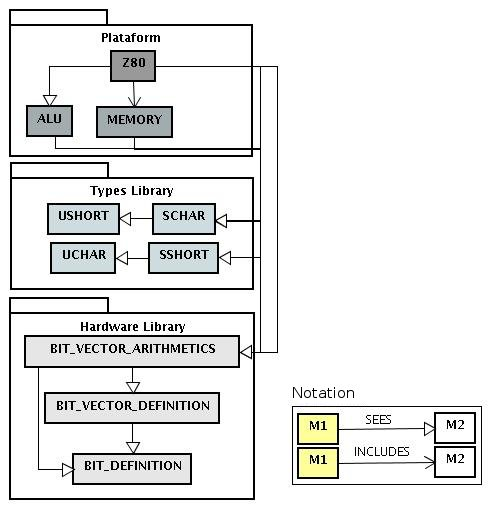
\includegraphics[width=.7\textwidth]{diagramaEstrutural.jpg}
\caption{Dependencies between modules of $\mathit{HARDWARE\_LIBRARY}$ and
platform model.}
\label{fig:hardware-definition-graph}

\end{figure}

Now, We will explain each of these modules and present them in detail.

\subsection{Definitions to represent and manipulate bits}

The entities defined in the module $\mathit{BIT\_DEFINITION}$ are the
type for bits, logical operations on bits (negation, conjunction,
disjunction, exclusive disjunction), as well as a conversion function
from booleans to bits.

First, bits are modeled as the set of integers $\{0, 1\}$:\\

$
\begin{array}{l}
\mathit{BIT} = \mathit{0..1} \\ 
\end{array}
$

The negation is a unary function on bits and it is defined as:

$
\begin{array}{l}
\mathit{bit\_not}  \in  \mathit{BIT}  \fun  \mathit{BIT}  \land \\
\forall ( \mathit{bb}). (\mathit{bb} \in \mathit{BIT} \implies \mathit{bit\_not}(\mathit{bb}) =
1-\mathit{bb})\\
\end{array}
$

The module also provides lemmas on negation that may be useful for the
users of the library to develop proofs:

$
\begin{array}{l}
 \mathit{bit\_not}(0) = 1;  \mathit{bit\_not}(1) = 0; \\
\forall (\mathit{bb}).(\mathit{bb} \in \mathit{BIT} \implies \mathit{bit\_not}(\mathit{bit\_not}(\mathit{bb})) = \mathit{bb});
\end{array}
$

Conjunction is a unary function on bits and it is defined as:

$
\begin{array}{l}
\mathit{bit\_and} \in \mathit{BIT} \times \mathit{BIT} \fun \mathit{BIT} \land \\
\forall (\mathit{b1}, \mathit{b2}).(\mathit{b1}  \in \mathit{BIT}  \land \mathit{b2} \in \mathit{BIT} \implies \\
\quad ((\mathit{bit\_and}(\mathit{b1}, \mathit{b2}) = 1) \iff (\mathit{b1} = 1)  \land  (\mathit{b2} = 1)))
\end{array}
$

The module provides the following lemmas for conjunction, either:

$
\begin{array}{l}
 \mathit{bit\_and}(0,0) = 0;  \mathit{bit\_and}(0,1) = 0; \\
 \mathit{bit\_and}(1,0) = 0;  \mathit{bit\_and}(1,1) = 1; \\
\forall (\mathit{b1},\mathit{b2}).(\mathit{b1} \in \mathit{BIT} \land \mathit{b2} \in \mathit{BIT} \implies \\
\quad (\mathit{bit\_and}(\mathit{b1}, \mathit{b2}) = \mathit{bit\_and}(\mathit{b2},\mathit{b1}))); \\
\forall (\mathit{b1},\mathit{b2},\mathit{b3}).(\mathit{b1} \in \mathit{BIT} \land  \mathit{b2} \in \mathit{BIT} \land \mathit{b3} \in \mathit{BIT} \implies \\
\quad (\mathit{bit\_and}(\mathit{b1}, \mathit{bit\_and}(\mathit{b2},\mathit{b3})) = \mathit{bit\_and}(\mathit{bit\_and}(\mathit{b1},\mathit{b2}),\mathit{b3}))); \\
\forall (\mathit{b1}).(\mathit{b1} \in \mathit{BIT} \implies (\mathit{bit\_and}(\mathit{b1}, 1) = \mathit{b1})); \\
\forall (\mathit{b1}).(\mathit{b1} \in \mathit{BIT} \implies (\mathit{bit\_and}(\mathit{b1}, 0) = 0));
\end{array}
$

The module provides definitions of $\mathit{bit\_or}$ (disjunction) and $\mathit{bit\_xor}$ (exclusive disjunction),
as well as lemmas on those operators. These are standard and their expression in B is similar as for
$\mathit{bit\_and}$, they are thus omitted.


Finally, the conversion from booleans to bits is simply defined as:

$
\begin{array}{l}
\mathit{bool\_to\_bit} \in \BOOL \fun \mathit{BIT} \land \mathit{bool\_to\_bit} = \{ \TRUE \mapsto 1, \FALSE \mapsto 0 \} \\
\end{array}
$

Observe that all the lemmas that are provided in this module have been
mechanically proved by the theorem prover included with our B
development environment. None of these proofs requires human insight.


\subsection{Representation and manipulation of bit vectors}

Sequences are pre-defined in B, as functions whose the domain is an integer range with lower bound 1 (one). Indices
in bit vectors usually range from 0 (zero) upwards and the model we propose obeys this convention by making an
one-position shift where necessary.  We thus define bit vectors as non-empty sequences of bits, and
$\mathit{BIT\_VECTOR}$ is the set of all such sequences:



$
\begin{array}{l}
\mathit{BIT\_VECTOR} = \seq (\mathit{BIT})
\end{array}
$

The function $\mathit{bv\_size}$ returns the size of a given bit vector. It is basically a wrapper for the
predefined function $\mathbf{size}$ that applies to sequences.


$
\begin{array}{l}
\mathit{bv\_size} \in \mathit{BIT\_VECTOR} \fun \nat_1 \land \\
\mathit{bv\_size} = \lambda bv \bullet (bv \in \mathit{BIT\_VECTOR} \mid \mathbf{size}(bv))
\end{array}
$

We also define two functions $\mathit{bv\_set}$ and $\mathit{bv\_clear}$ that, given a bit vector, and a position of
the bit vector, return the bit vector resulting from setting the corresponding position to 0 or to 1, and a function
$\mathit{bv\_get}$ that, given a bit vector, and a valid position, each one returns the value of the bit at that
position. Only the first definition is shown here:


$
\begin{array}{l}
\mathit{bv\_set} \in \mathit{BIT\_VECTOR} \times \nat \fun \mathit{BIT\_VECTOR} \land \\
\mathit{bv\_set} = \lambda v, n \bullet (v \in \mathit{BIT\_VECTOR} \land 0 \in \nat \land n < \mathit{bv\_size}(v) \mid v \ovr \{ n+1 \mapsto 1 \})
\end{array}
$

The function $bv\_catenate$ takes as parameters two bit vectors $v$ and $w$, and returns the result of the
concatenation of $v$ and $w$, such that $v$ constitutes the most significant part of the result.


% $
% \begin{array}{l}
% \mathit{bv\_catenate} \in \mathit{BIT\_VECTOR} \times \mathit{BIT\_VECTOR} \fun \mathit{BIT\_VECTOR} \land \\
% \mathit{bv\_catenate} = \lambda v, w \bullet (v \in \mathit{ BIT\_VECTOR} \land w \in \mathit{ BIT\_VECTOR}  \mid v 
% %\conc
%   w)
% \end{array}
% $


\hspace*{0.00in} \it bv\_catenate  $\in$  \it BIT\_VECTOR  $\times$  \it BIT\_VECTOR  $\fun$ \it BIT\_VECTOR $\land$ 

\hspace*{0.00in} \it bv\_catenate \rm =  $\lambda$  v\rm ,\it w \rm . \rm (\it v  $\in$  \it BIT\_VECTOR $\land$ \it w $\in$  \it BIT\_VECTOR  $\mid$  \it v $\cat$ \it w\rm )




We also define a function $\mathit{bv\_zero}$ that, given a positive
integer $n$, return a bit vector of size $n$, with all bits set to 0.
A similar function, called $\mathit{bv\_one}$, with all bits set to 1
is also defined but not presented here.

$
\begin{array}{l}
\mathit{bv\_zero} \in \nat_1 \fun \mathit{BIT\_VECTOR} \land \\
\mathit{bv\_zero} = \lambda n \bullet (n \in \nat_1 \mid 1..n \times \{0\}) 
\end{array}
$

Additionally, the module provides definitions for the classical
logical combinations of bit vectors: $\mathit{bit\_not}$,
$\mathit{bit\_and}$, $\mathit{bit\_or}$ and $\mathit{bit\_xor}$. Only
the first two are presented here. Observe that the domain of the
binary operators is restricted to pairs of bit vectors of the same
length:

$
\begin{array}{l}
\mathit{bv\_not} \in \mathit{BIT\_VECTOR} \fun \mathit{BIT\_VECTOR} \land \\
\mathit{bv\_not} = \lambda v \bullet (v \in \mathit{BIT\_VECTOR} \mid \\
\quad \lambda i \bullet 0 .. \mathit{bv\_size}(v)-1 \mid \mathit{bit\_not}(v(i))) \land \\
\mathit{bv\_and} \in \mathit{BIT\_VECTOR} \times \mathit{BIT\_VECTOR} \fun \mathit{BIT\_VECTOR} \land \\
\mathit{bv\_and} = \lambda v_1, v_2 \bullet (v_1 \in \mathit{BIT\_VECTOR} \land v_2 \in \mathit{BIT\_VECTOR} \land \\
\quad \mathit{bv\_size}(v_1) = \mathit{bv\_size}(v_2) \mid \lambda i \bullet 0 .. \mathit{bv\_size}(v_1)-1 \mid \mathit{bit\_and}(v_1(i), v_2(i)))
\end{array}
$

We provide several lemmas on bit vector operations. These lemmas
express properties on the size of the result of the operations
as well as classical algebraic properties such as associativity
and commutativity. For example:

$
\begin{array}{l}
\forall v \bullet (v \in \mathit{BIT\_VECTOR} \implies \mathit{bv\_size}(\mathit{bv\_not}(v)) = \mathit{bv\_size}(v)) \\

\forall v \bullet (v \in \mathit{BIT\_VECTOR} \implies \mathit{bv\_not}(\mathit{bv\_not}(v)) = v) \\

\forall v_1, v_2 \bullet (\{v_1, v_2\} \subseteq \mathit{BIT\_VECTOR} \land \mathit{bv\_size}(v_1) = \mathit{bv\_size}(v_2) \implies \\
\quad \mathit{bv\_size}(\mathit{bv\_and}(v_1, v_2)) = \mathit{bv\_size}(v_1)) \\

\forall v_1, v_2 \bullet (\{v_1, v_2\} \subseteq \mathit{BIT\_VECTOR} \land \mathit{bv\_size}(v_1) = \mathit{bv\_size}(v_2) \implies \\
\quad \mathit{bv\_size}(\mathit{bv\_and}(v_1, v_2)) = \mathit{bv\_size}(v_2)) \\

\forall v_1, v_2 \bullet (\{v_1, v_2\} \subseteq \mathit{BIT\_VECTOR} \land \mathit{bv\_size}(v_1) = \mathit{bv\_size}(v_2) \implies \\
\quad \mathit{bv\_size}(\mathit{bv\_and}(v_1, v_2)) = \mathit{bv\_and}(v_2, v_1)) \\

\forall v_1, v_2, v_3 \bullet (\{v_1, v_2, v_3\} \subseteq \mathit{BIT\_VECTOR}
\land \mathit{bv\_size}(v_1) = \mathit{bv\_size}(v_2) \land \\
\quad \mathit{bv\_size}(v_1) = \mathit{bv\_size}(v_3) \implies \\ 
\quad \mathit{bv\_and}(\mathit{bv\_and}(v_1, v_2), v_3) = \mathit{bv\_and}(v_1,
\mathit{bv\_and}(v_2, v_3))) \\

\forall v \bullet (v \in \mathit{BIT\_VECTOR} \implies \\
\quad \mathit{bv\_and}(v, \mathit{bv\_zero}(\mathit{bv\_size}(v))) = \mathit{bv\_zero}(\mathit{bv\_size}(v))) \\

\forall v \bullet (v \in \mathit{BIT\_VECTOR} \implies \\
\quad \mathit{bv\_and}(v, \mathit{bv\_one}(\mathit{bv\_size}(v))) = v) \\

\end{array}
$

\subsection{Modelling bytes}

Bit vectors of length 8 are bytes. They form a common entity in
hardware design. We provide the following definitions:

$
\begin{array}{l}
\mathit{BYTE\_WIDTH} = 8 \land \mathit{BYTE\_INDEX} = 0..(\mathit{BYTE\_WIDTH}-1) \land \\
\mathit{BYTE} \subseteq \mathit{BIT\_VECTOR} \land \mathit{BYTE} = \{ v \in \mathit{BIT\_VECTOR} \land \mathit{bv\_size}(v) = \mathit{BYTE\_WIDTH}\} \land \\
\mathit{BYTE\_ZERO} \in \mathit{BYTE} \land \mathit{BYTE} = \mathit{BYTE\_INDEX} \times \{0\} 
\end{array}
$

\subsection{Bit vector arithmetics}

Bit vectors are used to represent and combine numbers: integer ranges
(signed or unsigned) and floating point numbers.

Our library defines a function $\mathit{bv\_to\_nat}$ that maps bit
vectors to natural numbers:

$
\begin{array}{l}
\mathit{bv\_to\_nat} \in \mathit{BIT\_VECTOR} \fun \nat \land \\
\mathit{bv\_to\_nat} = \lambda v \bullet (v \in \mathit{BIT\_VECTOR} \mid \sum i \bullet (i \in \dom(v) \bullet v(i) \times 2^i))
\end{array}
$

We provide the following lemma:

$
\begin{array}{l}
\forall n \bullet (n \in \nat_1 \implies \mathit{bv\_to\_nat}(\mathit{bv\_zero}(n)) = 0)
\end{array}
$

\subsection{Basics data types}

There are data types commonly used in the microcontrollers. They are placed in
the project Types Librarys and define functions to manipulate data on levels of
basic types from hardware. However, in general is needed to detail or redefines
the types and its functions for each platform. Then, the specific concepts are
defined in the project's own platform.

There are six common basics data types, see details in table below.

\begin{tabular}{|p{3.5cm}|c|c|c|}\hline
 $Type\ Name$ & $Range$ & $Physical\ Size $\\ 
\hline
 UCHAR& 0..255 & 1 byte\\ \hline SCHAR& -128..127 & 1 byte\\ \hline BYTE & -- & 1
 byte\\ \hline USHORTINT & 0..65.535 & 2 byte\\ \hline SSHORTINT &
 -32.768..32.767 & 2 byte\\ \hline BV16 & -- & 2 byte\\ \hline
\end{tabular} 


There is, for example, the function $\mathit{bv\_to\_nat}$ that is specialized
to $\mathit{byte\_uchar}$. How the set $\mathit{BYTE}$ is a subset of the
$\mathit{BIT\_VECTOR}$, then this function can defined as follows:

$
\begin{array}{l}
\mathit{byte\_uchar} = \lambda (v) \bullet ( v \in BYTE | bv\_nat(v) )
\end{array}
$

Usually, the definitions of the functions of the module $\mathit{TYPES}$ are the
re-used from the basic functions of the hardware library. This provides greater
confidence and facilitates the process of proof, because the prover can use the
defined previous lemma.

A more specific model of $\mathit{byte\_uchar}$ functions is:

$
\begin{array}{l}
\mathit{byte\_uchar} \in \mathit{BYTE}  \fun  \mathit{UCHAR}  \land \\
   \mathit{byte\_uchar} =  \lambda ( v0 )  \bullet  
   ( v0 \in \mathit{BYTE} |  2^{7}* bv\_get( v0 ,7 ) + 2^{6} * bv\_get( v0 ,6 ) + 2^{5}* bv\_get( v0 , 5   )\\ 
   + 2^{4}* bv\_get( v0 , 4 ) + 2^{3}*bv\_get( v0 , 3 ) + 2^{2}* bv\_get( v0 , 2 ) + 2 * bv\_get( v0 , 1 ) +  bv\_get( v0 ,0) )
   
\end{array}
$

The inverse function is easily defined as $\mathit{uchar\_byte}$.

$
\begin{array}{l}
\mathit{uchar\_byte} \in \mathit{UCHAR}  \fun  \mathit{BYTE}  \land \\
   \mathit{uchar\_byte} = \  ^{-1}(\mathit{byte\_uchar}
   )
\end{array}
$ 

We also created the following lemmas:
 
$
\begin{array}{l}
 \forall (val) \bullet (val \in \mathit{UCHAR} |
 \mathit{byte\_uchar}(\mathit{uchar\_byte}(val)) = val) \land\\
 \forall (by) \bullet (by \in \mathit{BYTE} |
 \mathit{uchar\_byte}(\mathit{byte\_uchar}(by)) = by)
\end{array}
$ 

Similarly, several other functions and lemmas were created for all other
data types.
		


\section{Description of the B model from Z80}
\label{sec:z80}

The \textit{Z80} is an important microcontroller developed in 1976 by \textit{Zilog}. In this time, It got a great
acceptance because suported all set instruction of \textit{8080}, one of the predecessors of the \textit{Pentium}
from \textit{Intel Corporation}. Then, the Z80 has the set instructions similar to the x86 architecture, it helps 
to build the model of x86 and it provides good features.


The main module includes a instance of memory module and accesses the definitions from: basic data types modules,
$\mathit{ALU}$ and $\mathit{Power2}$ \footnote{The $\mathit{Power2}$ module has the basics definitions to help the
theorems prover about calculus of power.}.

\begin{sloppypar}

\bf MACHINE

\hspace*{0.15in}\it Z80

\bf INCLUDES

\hspace*{0.10in}\it MEMORY

\bf SEES

\hspace*{0.10in}\it ALU, \it BIT\_DEFINITION, \it BIT\_VECTOR\_DEFINITION,

\hspace*{0.10in}\it BYTE\_DEFINITION, \it BV16\_DEFINITION, 

\hspace*{0.10in}\it UCHAR\_DEFINITION, \it SCHAR\_DEFINITION,

\hspace*{0.10in}\it SSHORT\_DEFINITION ,\it USHORT\_DEFINITION, \it POWER2
\end{sloppypar}


% Chacteristics of microcontroller
The \textit{Z80} supports 158 differents instructions including all the 78 from
\textit{8080}.The instructions are classified into these categories: load and exchange;
block transfer and search; arithmetic and logical; rotate and shift; bit
manipulation (set, reset, test); jump, call and return; input/output; and basic
cpu control. Each instruction and external action at model is represented by B
operations. By default, all parameters from operations are or pre-defined elements
in the model or integers values in the decimal representation.

The internal registers contain 208 bits of reading/writing memory. It includes two sets of six general purpose
registers which may be used individually as  8-bits registers or as 16-bits register pairs.  The work registers are
represented by variable $\mathit{rgs8}$. The domain of $\mathit{rgs8}$ ($\mathit{id\_regs8}$) is a set formed by
identifiers of registers of 8 bits. These registers can be accessed in pairs, forming 16-bits, resulting in other
set of identifiers of 16-bits registers, named $\mathit{id\_reg16}$. The main work register of Z80 is the
accumulator ($\mathit{rgs8(a0)}$) used for arithmetic, logic, input/output and loading/storing operations.



\begin{sloppypar}
\bf SETS

\hspace*{0.10in}\it id\_reg\_8 \rm = \rm \{ \it a0 \rm , \it f0 \rm , \it f\_0 \rm , \it a\_0 \rm ,

\hspace*{1.0 in}\it b0 \rm , \it c0 \rm , \it b\_0 \rm , \it c\_0 \rm ,

\hspace*{1.00in}\it d0 \rm , \it e0 \rm , \it d\_0 \rm , \it e\_0 \rm ,

\hspace*{1.0in}\it h0 \rm , \it l0 \rm , \it h\_0 \rm , \it l\_0 \} ;

\hspace*{0.10in}\it id\_reg\_16 \rm = \rm \{ \it BC \rm , \it DE \rm , \it HL \rm , \it SP \rm , \it AF \rm \}
\end{sloppypar}

\subsection{Modelling registers and input and output ports} [I need review the english]

The Z80 CPU includes alternative set of accumulator, flag and general registers. The CPU contains a stack
pointer ($\mathit{sp}$), program counter ($\mathit{pc}$), two index registers ($\mathit{ix}$ and $\mathit{iy}$), an
interrupt register ($\mathit{i\_}$), a refresh register ($\mathit{r\_}$), two bits ($\mathit{iff1}$,
$\mathit{iff2}$) used to control the interruptions, a pair of bits to define the interruption mode ($\mathit{im}$)
and the input and output ports ($\mathit{i\_o\_ports}$). Below, its definitions are represented by
\textit{INVARIANT}.
  
\begin{sloppypar}
\bf INVARIANT


\hspace*{0.10in}\it rgs8  $\in$  \it id\_reg\_8  $\fun$  \it BYTE  $\land$ 

\hspace*{0.10in}\it pc  $\in$  \it INSTRUCTION  $\land$  \it sp  $\in$  \it BV16  $\land$  \it ix  $\in$  \it BV16  $\land$  \it iy  $\in$  \it BV16  $\land$ 

\hspace*{0.10in}\it i\_  $\in$  \it BYTE  $\land$  \it r\_\hspace*{0.10in} $\in$  \it BYTE  $\land$  

\hspace*{0.10in}\it iff1  $\in$  \it BIT  $\land$ \hspace*{0.10in}\it iff2  $\in$  \it BIT  $\land$ 

\hspace*{0.10in}\it im \rm : \rm (\it BIT $\times$ \it BIT\rm )  $\land$ 

\hspace*{0.10in}\it i\_o\_ports  $\in$  \it BYTE  $\fun$  \it BYTE
\end{sloppypar}

\subsection{Flag register} [I need review the english]
Another important element is the ``z'' register ($\mathit{rgs8(z0)}$),  that is used as a flag register. This
register uses only six bits to represent the result status of each instruction. 	
According to the official manual the bits 3 and 5 are not used and the others bits have the follow meaning:
\begin{description}
  \item[$\mathit{bv\_get(rgs8(z0),0)}$] - The Carry bit
  \item[$\mathit{bv\_get(rgs8(z0),1)}$] - The Add/Subtract bit
  \item[$\mathit{bv\_get(rgs8(z0),2)}$] - The Parity or Overflow bit
  \item[$\mathit{bv\_get(rgs8(z0),4)}$] - The Half Carry bit
  \item[$\mathit{bv\_get(rgs8(z0),6)}$] - The Zero bit
  \item[$\mathit{bv\_get(rgs8(z0),7)}$] - The Sign bit 
\end{description}


\subsection{Manipulation data functions from Z80} [I need review the english] There are some specific functions from
Z80 to manipulate the data. The $\mathit{bv\_ireg\_plus\_d}$ is  used to indexed address. It received the
value of register ($\mathit{ix}$ or $\mathit{iy}$) and displacement to return the sum, the result is the memory address dislocated, see
its the definition.

\hspace*{0.0in}\it bv\_ireg\_plus\_d \rm : \rm(\it BV16  $\times$  \it SCHAR  $\fun$  \it BV16\rm )  $\land$ 

\hspace*{0.0in}\it bv\_ireg\_plus\_d \rm =  $\lambda$  \rm ( \it ix\_iy \rm , \it disloc \rm ) \rm . \rm ( \it ix\_iy  $\in$  \it BV16  $\land$  \it disloc  $\in$  \it SCHAR   

\hspace*{0.20in}$\mid$ \it ushort\_bv16 \rm ( \rm (\it bv16\_ushort \rm ( \it ix\_iy \rm ) \rm + \it disloc \rm ) 
$\mod$ \rm 6\rm 5\rm 5\rm 3\rm 6 \rm ) \rm )

Another derived function is  $\mathit{bv\_9ireg\_plus\_d0}$ , this returns the value in the memory  address
returned by $\mathit{bv\_ireg\_plus\_d}$ function ands its definition is similar.

There is a specific function to refresh the flag register, it is named $\mathit{update\_reg\_flag}$. It is typed of
follow mode: \it update\_flag\_reg \rm $\in$ \rm (\it BIT  $\times$  \it BIT  $\times$  \it BIT  $\times$  \it
BIT $\times$  \it BIT  $\times$  \it BIT\rm) $\fun$  \rm (\rm \{\it f0\rm \}  $\times$  \it BYTE\rm ). 

\it update\_flag\_reg \rm =  $\lambda$  \rm (\it s7 \rm, \it z6 \rm,\it h4 \rm,\it pv2 \rm ,\it n1
\rm ,\it c0 \rm)$\bullet$

\rm ( \it s7 $\in$ \it BIT $\land$ \it z6 $\in$ \it BIT $\land$ \it h4 $\in$ \it
BIT $\land$ \it pv2 $\in$ \it BIT $\land$ \it n1 $\in$ \it BIT $\land$ \it c0 $\in$ \it BIT
  
\hspace*{0.20in}\rm $\mid$( \it f0  $\mapsto$  \rm \rm [\it c0\rm , \it n1\rm , \it pv2\rm , \rm 1\rm , \it
h4\rm , \rm 1\rm , \it z6\rm , \it s7\rm \rm ]\rm ) \rm )


\subsection{Program, stack and data memory}[I need review the english]

The Z80 uses a unique memory for storing program instructions, data stack and data work. The memory has 16-bits
addressing and each address represent a byte. Thus, the data from the memory module is very simple, as shown below,
but an additional care must be taken to preserve the consistency of memory.

\begin{sloppypar}
\bf INVARIANT \\
\hspace*{0.10in}\it mem  $\in$  \it BV16  $\fun$  \it BYTE 

\end{sloppypar}
  
In general, the instructions can access all memory address, but it is very dangerous. For add more security, is
importante that the program instructions has the access limited by region. Thus, the designer can specify address
regions to restrict the access from instructions. The address regions can be especified how shown below.

$
\begin{array}{l}
\mathit{PROGRAM\_R\_ADR} = 0..16384 \land \mathit{DATA\_R\_ADR} = 16385..49151 \land \\
\mathit{STACK\_R\_ADR} = 49152..65535
\end{array}
$

\begin{property}[Assuring the absence of overlapping of address regions]
 To assure that address regions are well defined, then the designer must to verify the below expression.
\end{property}

\begin{sloppypar}
\hspace*{0.10in}\it PROGRAM\_R\_ADR $\cap$ DATA\_R\_ADR $\cap$  STACK\_R\_ADR $=$ \{\}
\end{sloppypar}
 


\begin{property}[Preserving the consistency of the memory]
In general, the access to some address regions is dangerous. Then, in each instruction has a specific
pre-condition that verify if the new address memory, that will be updated, is member of its region. For example,
the $\mathit{PUSH}$ program instruction allow write only in the region of stack ($\mathit{STACK\_R\_ADR}$). 
%Thus,if the user try to write in incorrect region then the called of operation cannot be proved.
\end{property}


\subsection{Arithmetic logic unit}
 
There are many functions defined in the module ALU. In general, these functions take basic definitions to build
new specific functions. The function half8UCHAR is used to get the half part of UCHAR value. It is importante to
know the half carry and it is used in the $\mathit{add8UCHAR}$. 

\hspace*{0.0in}

\hspace*{0.0in}\it half8UCHAR  $\in$  \it UCHAR  $\fun$  \it UCHAR  $\land$ 

\hspace*{0.0in}\it half8UCHAR \rm =  $\lambda$  \rm (\it ww\rm )\rm .\rm (\it ww  $\in$  \it UCHAR  $\mid$  \it ww  $\mod$  \it $2^{4}$\rm )

\hspace*{0.0in}

 
The function $\mathit{add8UCHAR}$ receive a bit carry and two $\mathit{UCHAR}$ values and return respectively the 
sum, the sign bit, the carry bit, the half carry bit and the zero bit. It is typed how follow: \it add8UCHAR \rm :
\rm (\it BIT $\times$ \it UCHAR $\times$ \it UCHAR\rm ) $\fun$ \rm (\it UCHAR $\times$  \it BIT  $\times$  \it BIT  $\times$  \it BIT  $\times$  \it BIT\rm ) and its definitions is:


\hspace*{0.20in}

\hspace*{0.0in}\it add8UCHAR\rm = $\lambda$ \rm(\it carry\rm,\it w1\rm \it w2\rm)\rm.\rm

\hspace*{0.0in}(\it carry $\in$  \it BIT  $\land$  \it w1  $\in$  \it UCHAR  $\land$  \it w2  $\in$  \it
UCHAR $\mid$

\hspace*{0.40in}\rm(\rm(\rm(\it carry \rm + \it w1 \rm + \it w2 \rm )  $\mod$  \it $2^{8}$ \rm ),

\hspace*{0.40in}\it bool\_bit\rm ( \it carry \rm + \it uchar\_schar\rm (\it w1\rm ) \rm + \it uchar\_schar \rm (\it w2\rm ) $<$ \rm 0\rm ),

\hspace*{0.40in}\it bool\_bit\rm ( \it carry \rm + \it w1 \rm + \it w2 $>$ \it UCHAR\_MAX\rm )\rm ,

\hspace*{0.40in}\it bool\_bit\rm ( \it carry \rm + \it half8UCHAR\rm (\it w1\rm ) \rm + \it half8UCHAR\rm ( \it w2\rm )  $\geq$  \it $2^{4}$\rm )\rm,

\hspace*{0.40in}\it bool\_bit\rm ( \rm ( \rm (\it carry \rm + \it w1 \rm + \it w2 \rm )  $\mod$  \it $2^{8}$ \rm )\rm = \rm 0\rm )\rm )\hspace*{0.10in}\rm )

\hspace*{0.20in}

A similar function to subtract operation is $\mathit{substract8UCHAR}$. There are the same functions for the
$\mathit{SCHAR}$ type, they are respectively $\mathit{add8SCHAR}$ and $\mathit{substract8SCHAR}$, all these
functions are of 8 bits ($\mathit{BYTE}$) and defined similarly. In the same way, the arithmetic functions for 16 bits
($\mathit{BV16}$) are defined.

Other more simply functions also are typed and explained below: 

\begin{itemize}
  \item ALU \it inc  $\in$ \it BYTE $\fun$  \it BYTE \rm - It receives a byte and returns its decrement. There is a
  similar function named $\mathit{dec}$.

  \item ALU \it instruction\_next  $\in$  USHORT  $\fun$  USHORT \rm - It receives the pc actual
  value and return its increment.

  \item ALU \it is\_negative  $\in$  \it BYTE  $\fun$  \it BIT \rm - It returns 1 if the received
  byte is zero, otherwise returns 0.
   
  \item byte \it is\_zero $\in$ BYTE  $\fun$   BIT \rm - It returns 1 if the received byte is zero, otherwise
  returns 0.
  
  \item byte \it rotateright  $\in$  \it BYTE  $\fun$  \it BYTE \rm - It receives a byte and returns its rotated to
  right. There is a similar function named $\mathit{rotateleft}$.  

  \item ALU \it update\_refresh\_reg \rm - It receives a byte and returns its increment until the seventh bit.
\end{itemize}
Every logic functions defined in the $\mathit{BYTE}$ module are included in the $\mathit{ALU}$ module. Then, it was
not necessary rewrite these functions.

\subsection{Interrupts}

% Vis�o Geral
In the Z80, the interrupts allows that the devices suspend a routine from CPU and start another service routine.
This service routine can exchange data or signals between CPU and external devices. When a routine is finished, then
the CPU come back to the last routine that was interrupted.

For the interrupts, the following things are important:  the interrupt flip-flops ($\mathit{iff1}$ and
$\mathit{iff2}$), the types of interrupts (maskable and non-maskable), the interrupt mode (set with the $\mathit{IM
0}$, $\mathit{IM 1}$, $\mathit{IM 2}$ instructions) and the $\mathit{i\_}$ register.

The $\mathit{iff1}$ and $\mathit{iff2}$ control the maskable interrupts ($\mathit{INT}$). When the $\mathit{iff1}$
is set, the interrupt is enable, otherwise it is disable. The $\mathit{iff2}$ is used only as a tempory storage
place for $\mathit{iff1}$. The $\mathit{iff1}$ is set or reset by instructions $\mathit{EI}$ and $\mathit{DI}$.


The interruptions and the \textit{reset} action change the state of
microcontroller. Theses actions are modeled by B operations and the its main
effects are shown below\footnote{Some definitions: $\mathit{sp\_minus\_two}$ =
$\mathit{dec\_BV16(dec\_BV16(sp))}$, $\mathit{sp\_minus\_one}$=
$\mathit{dec\_BV16(sp)}$, $\mathit{pc\_high}$ is the most significant 8 bits and
$\mathit{pc\_low}$ is the least significant. }.


 \textbf{NMI} - Non-maskable interrupts - The non-maskable cannot be disable
 by the programmer. Then, when a device makes a request, the $sp$ is pushed, the $pc$ receive
 $66H$ (102 in decimal), the $\mathit{iff1}$ is reset , $\mathit{iff2}$ stores
 $\mathit{iff1}$ and refresh register is updated.
  
% $updateStack(\{ (sp\_minus\_two \fun low\_pc ),(sp\_minus\_one
%    \fun high\_pc ) \}) ||\\  sp:= sp\_minus\_two || pc := 66H || iff1:=0 || 
%    iff2:= iff1 $
\begin{sloppypar}
\bf updateStack\rm (\rm \{ \rm (\it sp\_minus\_two  $\mapsto$  \it pc\_low\rm )\rm ,\rm (\it sp\_minus\_one  $\mapsto$ \it pc\_high \rm ) \rm \}\rm )$\para$

\it sp \rm := \it sp\_minus\_two  $\para$ \it pc \rm := \rm 1\rm 0\rm 2 $\para$ \it iff1\rm :=\rm 0  $\para$  \it iff2\rm := \it iff1 $\para$

\it r\_ \rm := \it update\_refresh\_reg\rm (\it r\_\rm )\\
\end{sloppypar}

  \textbf{INT} - Maskable Interrupt -  This is usualy reserved to important functions that can be enabled and
  disabled by the programmer. When a maskable interrupt action happens, both $\mathit{iff1}$ and $\mathit{iff2}$ are
  cleared, disabling the interrupts, the $sp$ is pushed, the refresh register is updated  and the other effects
  depend on the interrupt mode.
 

 \begin{itemize}
   
  \item The mode 0 is compatible with 8080 and  \it im \rm = \rm ( \rm 0 $\mapsto$  \rm 0 \rm ). When a 
  non-maskable interruption happen , the CPU fetches an instruction of one byte from an external device, usually an
  RST instruction, and the CPU executes it. The instruction code is received from a external device by data bus and
  it is represented by integer parameter called $\mathit{byte\_bus}$ .

 
   \item The mode 1 is the easiest and \it im \rm = \rm ( \rm 0  $\mapsto$  \rm 1 \rm ). Simply, when a non-maskable
   interruption happens, the program counter receive $38H$ (56 in decimal).
  
   \item The mode 2 is the most powerfull and  \it im \rm = \rm ( \rm 1  $\mapsto$ \rm 1 \rm ). When a non-maskable
   interruption happens, an indirect call can be made to any address memory. The program counter receives in the
   part most significant the $\mathit{i\_}$ register and, in the  part least siginificant, the $\mathit{byte\_bus}$
   with the last bit reset.
 \end{itemize}

The essential part of maskable interrupt is shown below\footnote{ The
 $\mathit{byte\_bus}$ is parameter from  $\mathit{INT}$ operation }. 
 


\begin{sloppypar}

\hspace*{0.00in}\bf IF \it im \rm = \rm ( \rm 0  $\mapsto$  \rm 0 \rm ) \bf THEN  

\hspace*{0.10in}\bf IF\hspace*{0.10in}\it byte\_bus \rm $\in$  \it opcodes\_RST\_instruction

\hspace*{0.10in}\bf THEN\hspace*{1.05in}

\hspace*{0.40in}\it pc \rm := \it byte\_bus \rm - \rm 1\rm 9\rm
9\hspace*{0.10in} $\para$

\hspace*{0.40in}\bf updateStack\rm ( \rm \{ \it stack\rm ( \it
sp\_minus\_one\rm )  $\mapsto$  \it pc\_low\rm ,

\hspace*{0.40in}\it stack\rm (\it sp\_minus\_two\rm )  $\mapsto$  \it pc\_high
\rm \} \rm )  $\para$

\hspace*{0.40in}\it sp \rm := \it sp\_minus\_two  $\para$ \hspace*{0.10in}\it
r\_ \rm := \it update\_refresh\_reg\rm (\it r\_\rm )

\hspace*{0.10in}\bf ELSIF \it byte\_bus \rm = \it opcode\_\ldots\_instruction

\hspace*{0.40in}\bf \ldots 

\hspace*{0.10in}\bf END

\hspace*{0.00in}\bf ELSIF\hspace*{0.10in}\it im \rm =\hspace*{0.10in}\rm ( \rm
0  $\mapsto$  \rm 1 \rm ) \bf THEN

\hspace*{0.10in}\it pc \rm :=\hspace*{0.10in}\rm 5\rm 6  \hspace*{0.80in}
$\para$

\hspace*{0.10in}\bf updateStack\rm ( \rm \{ \it stack\rm (\it
sp\_minus\_one\rm )  $\mapsto$  \it pc\_low\rm ,

\hspace*{0.10in}\it stack\rm (\it sp\_minus\_two\rm )  $\mapsto$  \it pc\_high
\rm \} \rm )  $\para$

\hspace*{0.10in}\it sp \rm := \it sp\_minus\_two  $\para$ \hspace*{0.10in}\it
r\_ \rm := \it update\_refresh\_reg\rm (\it r\_\rm )\hspace*{0.85in}

\hspace*{0.00in}\bf ELSIF\hspace*{0.10in}\it im \rm = \rm ( \rm 1  $\mapsto$ 
\rm 1 \rm ) \bf THEN  \hspace*{0.70in}

\hspace*{0.10in}\it pc \rm := \it bv16\_ushort\rm (\it byte\_bv16\rm ( \it i\_
\rm ,\it bv\_clear\rm (\it rotateleft\rm (\it uchar\_byte\rm (\it byte\_bus\rm )\rm )\rm ,\rm 0\rm )\rm )\rm )$\para$

\hspace*{0.10in}\bf updateStack\rm ( \rm \{ \it stack\rm ( \it
sp\_minus\_one\rm )  $\mapsto$  \it pc\_low\rm ,

\hspace*{0.10in}\it stack\rm (\it sp\_minus\_two\rm )  $\mapsto$  \it pc\_high
\rm \} \rm )  $\para$

\hspace*{0.10in}\it sp \rm := \it sp\_minus\_two  $\para$ \hspace*{0.10in}\it
r\_ \rm := \it update\_refresh\_reg\rm (\it r\_\rm )

\hspace*{0.00in}\bf END\hspace*{0.10in}\\
\end{sloppypar}



\textbf{RESET}  - The reset is other external action that just reset the
registers related to the interruptions.

\begin{sloppypar}
\it iff1 \rm :=\rm 0 $\para$ \it iff2\rm :=\rm 0 $\para$  \it  im\rm := \rm (\rm 0 $\mapsto$ \rm 0\rm )  $\para$ 
\it pc\rm :=\rm 0 $\para$ \it i\_ \rm := [0,0,0,0,0,0,0,0] $\para$

\it rgs8 \rm := \it rgs8  $\lover$  \rm \{ \rm (\it a0  $\mapsto$ \rm [0,0,0,0,0,0,0,0] , \rm (\it
f0 $\mapsto$ \rm [0,0,0,0,0,0,0,0] \rm \} $\para$

\it r\_  \rm := [0,0,0,0,0,0,0,0] $\para$ \it sp \rm := [0,0,0,0,0,0,0,0,0,0,0,0,0,0,0,0]
\end{sloppypar}


% 
%     Para controlar o registrador I, existem duas intrucoes:
% 
%     - LD A,I (carrega o acumulador com o valor contido em I);
%     - LD I,A (carrega I com o valor contido no acumulador).
% 
%     A instrucao LD A,I possui uma funcao extra, ja' discutida
% em outra aula: ela carrega na `flag' de paridade/sobrecarga o
% valor do IFF ("Interruption Flip-Flop"). Se IFF for 0, entao a
% interrupcao mascaravel esta' desativada. Se IFF for 1, entao
% ela esta' ativada.
% %%%% FIM - http://download.unesp.br/msx/asm/course_4.txt
% 
% 
% 
% 
% Instru��es relacionadas com o sistema de interrup��o:
%  HALT,EI,DI,M0,M1,M2 
%  
%  LD_A_R, LD_A_I\ldots,  
%  CALL, RET,  RETI,RETN






\subsubsection{I/O Ports} % Can be placed in basic definitions in a paragraph
%Referencia o modeo de modelagem do captura de um evento externo de acordo com
% o proposto em [DAVID_gdc_2007] 

[[ Flag registers and the associated functions: negative, half, zero.. ]] 

\section{Extern  actions and input and output ports}

The Z80 has an extensive set of input and output instruction and 256 ports for
devices. This model can transfer data blocks and between the I/O devices and any
of the internal registers or memory address.

The $\mathit{IN\_r(C)}$ \footnote{The tools B don't allow use parenteses in identifiers, then the characteres
\{``('',``)''\} are replaced respectively by \{``9'',``0''\} in the real specification.} is represented by the follow B
operation. This instruction is from I/O group and update the flag registers.

\hspace*{0.0in}\bf IN\_r\_(C) \rm ( \it rr \rm ) \rm =

\hspace*{0.0in}\bf PRE \it rr  $\in$  \it id\_reg\_8  $\land$  \it rr  $\not =$  \it f0\hspace*{0.15in}\bf THEN

\hspace*{0.20in}\bf ANY

\hspace*{0.40in}\it negative \rm , \it zero \rm , \it half\_carry \rm , \it pv \rm , \it add\_sub \rm , \it carry

\hspace*{0.20in}\bf WHERE 

\hspace*{0.40in}\it negative $\in$ \it BIT $\land$ \it zero $\in$ \it BIT $\land$ \it half\_carry $\in$ \it BIT 
$\land$ \it pv $\in$ \it BIT $\land$

 \hspace*{0.40in}\it add\_sub $\in$ \it BIT $\land$ \it carry $\in$ \it BIT  $\land$

\hspace*{0.40in}\it negative \rm = \it is\_negative \rm ( \it io\_ports \rm ( \it rgs8 \rm ( \it c0 \rm ) \rm ) \rm )  $\land$ 

\hspace*{0.40in}\it zero \rm = \it is\_zero \rm ( \it io\_ports \rm ( \it rgs8 \rm ( \it c0 \rm ) \rm ) \rm )  $\land$ 

\hspace*{0.40in}\it half\_carry \rm = \rm 0  $\land$ 

\hspace*{0.40in}\it pv \rm = \it parity\_even \rm ( \it io\_ports \rm ( \it rgs8 \rm ( \it c0 \rm ) \rm ) \rm ) $\land$

\hspace*{0.40in}\it add\_sub \rm =\hspace*{0.10in}\rm 0  $\land$ 

\hspace*{0.40in}\it carry \rm = \it z\_c

\hspace*{0.20in}\bf THEN

\hspace*{0.40in}\it rgs8 \rm := \it rgs8  $\lover$  \rm \{ \rm ( \it rr  $\mapsto$  \it io\_ports \rm ( \it rgs8 \rm ( \it c0 \rm ) \rm ) \rm ) \rm ,

\hspace*{0.40in}\it update\_flag\_reg\rm (\it negative\rm,\it zero\rm,\it half\_carry\rm,\it pv\rm,\it add\_sub\rm,\it carry)\rm\}$\para$

\hspace*{0.40in}\it pc \rm := \it instruction\_next \rm ( \it pc \rm )  $\para$  \it r\_ \rm := \it update\_refresh\_reg\rm (\it r\_\rm )

\hspace*{0.0in}\bf END \rm



% $
% \begin{array}{l} 
% \mathit{IN\_r\_9C0} ( rr ) = \\
% \quad   \PRE rr \in id\_reg\_8    \THEN\\
% \quad\quad \ANY data\_in, negative , zero , half\_carry , pv , add\_sub , carry\\ 
% \quad\quad \WHERE data\_in \in \mathit{BYTE} \land negative \in \mathit{BIT}\land\\
% \quad\quad\quad carry \in \mathit{BIT} \land half\_carry \in \mathit{BIT} \land zero \in \mathit{BIT} \land \\
% \quad\quad\quad negative = is\_negative (data\_in) \land zero = is\_zero(data\_in ) \land\\
% \quad\quad\quad half\_carry = 0 \land pv =parity\_even\_BYTE ( data\_in )    \land\\
% \quad\quad\quad add\_sub =  0 \land carry = z\_c \\
% \quad\quad  \THEN \\
% \quad\quad\quad i\_o\_ports ( rgs8 ( c0 ) ) := data\_in ||\\
% \quad\quad\quad rgs8 := rgs8 <+ \{ ( rr |-> data\_in ) ,\\
% \quad\quad\quad get\_new\_flag\_register\_SZ\_H\_PvNC ( rgs8 , negative , zero, half\_carry , pv , add\_sub , carry ) \} ||\\
% \quad\quad\quad pc := instruction\_next( pc )\\
% \quad\quad \END\\
% \quad \END\\
% \end{array}
% $

\subsubsection{Instruction set} 
% Talk in general and put a example with midlle
% complex



 




 
 
 \section{Conlusitions}
 
%  Para a modelagen dessa plataforma, essa modelagen cont�m linhas e $np $
%  provas n�o obvias. Uma forma de acelerar o processo de prova, foi paralelizar
%  as provas. Isto foi feito em 4 IMacs e consumiu $ tp $ tempo para verificar
%  automaticamente $np - p $. As demais foi necess�rio uma certa intera��o com
%  o provador para sua verifica��o.
%  
%  
%  Algumas informa��es do manual do Z80 fornecido pela Zilog s�o imprecisas,
%  o que compremete um pouco a qualidade do modelo, entretanto alguns pontos
%  foram consultados no documento (Undocument Z80 documented-(Sean Young)) e
%  d�vidas foram sanadas com o uso do simulador(Z80 IDE Simulator). 
%  
%  Para oferecer uma maior garantia do modelo com a implementa��o do processador
%  algumas atividades foram realizadas. Primeiramente, tentantamos animar e gerar
%  c�digo respectivamente nas ferramentas ProB e AtelierB. Entratanto, o modelo
%  cot�m algumas constru��es complexas que ainda n�o s�o bem suportada por elas.
%  Ent�o, foi realizada uma apresenta��o sobre a descri��o do modelo e foi
%  realizada um nova revis�o com 3 pessoas.
 


\paragraph{Notes and Comments.}



% ---- Bibliography ----
%
\begin{thebibliography}{5}

\bibitem {Abrial}
Abrial, J. R. The B Book: Assigning Programs to Meanings. Cambridge University Press, United States of
America, 1 edition, 1996.

% Paper about BHDL 

% Paper of ALEM�O PROB ,java virtual machine

% Outros do artigo de bartira

% O manual do Z80 


\bibitem {Bell} 
 D. Bell, I. M. E. J. P. Software Engineering: A Programming Approach. Prentice Hall, New York, 2 edition, 1992.

\bibitem {Dantas}
 Dantas, B; D\'{e}harbe, D; Galv\~{a}o, S; ET AL. Proposta e avalia��o de uma abordagem de desenvolvimento de
 software fidedigno por constru��o com o m�todo B. In: SEMISH, Bel�m, 2008. SBC.

\end{thebibliography}

\end{document}
%
% \bibitem {clar:eke}
% Clarke, F., Ekeland, I.:
% Nonlinear oscillations and
% boundary-value problems for Hamiltonian systems.
% Arch. Rat. Mech. Anal. {\bf 78} (1982) 315--333
% %
% \bibitem {clar:eke:2}
% Clarke, F., Ekeland, I.:
% Solutions p\'{e}riodiques, du
% p\'{e}riode donn\'{e}e, des \'{e}quations hamiltoniennes.
% Note CRAS Paris {\bf 287} (1978) 1013--1015
% %
% \bibitem {mich:tar}
% Michalek, R., Tarantello, G.:
% Subharmonic solutions with prescribed minimal
% period for nonautonomous Hamiltonian systems.
% J. Diff. Eq. {\bf 72} (1988) 28--55
% %
% \bibitem {tar}
% Tarantello, G.:
% Subharmonic solutions for Hamiltonian
% systems via a $\bbbz_{p}$ pseudoindex theory.
% Annali di Matematica Pura (to appear)
% %
% \bibitem {rab}
% Rabinowitz, P.:
% On subharmonic solutions of a Hamiltonian system.
% Comm. Pure Appl. Math. {\bf 33} (1980) 609--633
% \end{thebibliography}
%

